\chapter{Pairwise space and Time series Metric Learning (TML) formalization}
\label{sec:TML}
\minitoc


%\noindent Chapeau introductif
%\begin{itemize}
%	\item Le calcul d'une métrique implique toujours 2 individus. On va proposer un changement d'espace, un nouvel espace : la représentation par paire.
%	\item Le cadre : on suppose que l'on a p métriques.
%\end{itemize}

\fbox{  \parbox{0.9\textwidth}{
		In this chapter, we formalize the problem of Time series Metric Learning ({\sc tml}) which is the learning of a metric that combines several unimodal metrics for a robust $k$-NN classifier. \\
		We first introduce a new space representation, the pairwise space. Secondly, we transpose the metric learning problem in the pairwise space. Finally, we propose three possible formulations: Linear programming, Quadratic programming and {\sc svm}-based approach.
	}  }

%---------------------------------------------------------------------------
\section{Pairwise space representation}
%\begin{itemize}
%	\item Changement de l'espace
%	\item Normalisation de l'espace des paires
%	\item Label des pairwise
%\end{itemize}
Let  $d_1, ..., d_h ..., d_p$ be $p$ given metrics that allow to compare samples. For instance, in Chapter \ref{sec:Chapter_metrics}, we have proposed three types of metrics for time series: amplitude-based $d_A$, behavior-based $d_B$ and frequential-based $d_F$. Our objective is to learn a metric $D$ that combines the $p$ metrics in order to optimize the performance of a $k$-NN classifier. Formally:
\begin{equation}
	D = f(d_1, \ldots , d_p)
\end{equation}
In this section, we first introduce a new space representation, the pairwise space. Then, we present how to define pairwise labels for classification and regression problem. Finally, we give some interpretations in the pairwise space. 


\subsection{Pairwise embedding}
\label{sec:Pairwise_embedding}
The computation of a metric $d$, and of course $D$, always takes into account a pair of samples $(\textbf{x}_i,\textbf{x}_j)$. We introduce a new space representation referred as the \textbf{pairwise space}. In this new space, illustrated in Fig. \ref{fig:PairwiseEmbedding}, a vector $\textbf{x}_{ij}$ represents a pair of time series $(\textbf{x}_i,\textbf{x}_j)$ described by the $p$ unimodal metrics $d_h$: $\textbf{x}_{ij}=[d_1(\textbf{x}_i,\textbf{x}_j), ..., d_p(\textbf{x}_i,\textbf{x}_j)]^T$. We denote $N$ the number of pairwise vectors $\textbf{x}_{ij}$ generated by this embedding.
%		\begin{equation*}		
%			\textbf{x}_{ij}
%			=
%			\begin{bmatrix}
%		        d_1(\textbf{x}_i,\textbf{x}_j) 	\\
%		        ... 			\\
%		       	d_p(\textbf{x}_i,\textbf{x}_j)
%		     \end{bmatrix}	    	     
%		\end{equation*}


\begin{figure}[h!]
	\begin{minipage}[b]{1.0\linewidth}
		\centering
		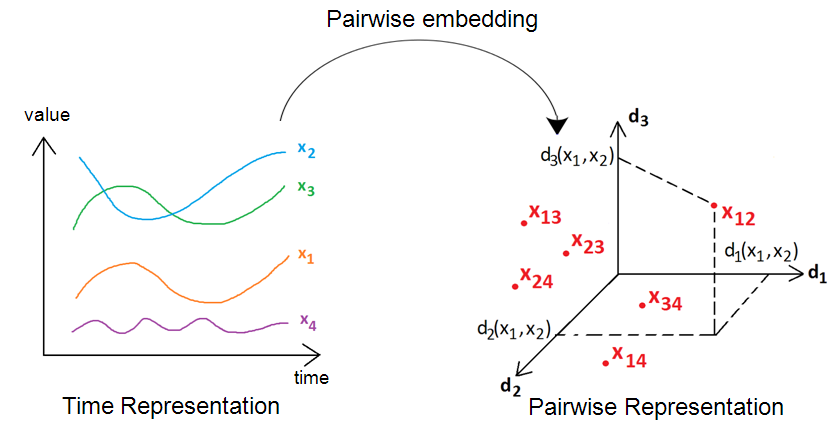
\includegraphics[width=0.9\linewidth]{images/PairwiseEmbedding}
	\end{minipage}
	\caption{Example of embedding of time series $\textbf{x}_i$ from the temporal space (left) into the pairwise space (right). In this example, a pair of time series $(\textbf{x}_1, \textbf{x}_2)$ is projected into the pairwise space as a vector $\textbf{x}_{12}$ described by $p=3$ basic metrics: $\textbf{x}_{12} = [d_1(\textbf{x}_1, \textbf{x}_2), d_2(\textbf{x}_1, \textbf{x}_2), d_3(\textbf{x}_1, \textbf{x}_2)]^T$.}
	\label{fig:PairwiseEmbedding}
\end{figure}

A combination function $D$ of the metrics $d_h$ can be seen as a function in this space. In the following, we propose first to use a linear combination of $d_h$: $D(\textbf{x}_i,\textbf{x}_j) = \sum_h w_h.d_h(\textbf{x}_i,\textbf{x}_j)$. For simplification purpose, we denote $D(\textbf{x}_i,\textbf{x}_j) = D(\textbf{x}_{ij})$ and the pairwise notation gives:
\begin{equation}
D(\textbf{x}_i,\textbf{x}_j) = D(\textbf{x}_{ij})=\textbf{w}^T\textbf{x}_{ij}
\label{eq:D_linear}
\end{equation}
where $\textbf{w}$ is the vector of weights $w_h$: $\textbf{w}=[w_1, \ldots, w_p]^T$.

\subsection{Pairwise label}
In the pairwise space, each vector $\textbf{x}_{ij}$ can be labeled $y_{ij}$ by following the rule: if $\textbf{x}_i$ and $\textbf{x}_j$ are similar, the vector $\textbf{x}_{ij}$ is labeled -1; and +1 otherwise. \\
For classification problems, the concept of similarity between samples $\textbf{x}_i$ and $\textbf{x}_j$ is driven by the class label $y_i$ and $y_j$ in the original space:
\begin{equation}
	y_{ij} = 
	\left\{
	\begin{split}
	-1 \text{\quad if } y_i = y_j\\ 
	+1 \text{\quad if } y_i \neq y_j
	\end{split}
	\right.
\end{equation}
For regression problems, each sample $\textbf{x}_i$ is assigned to a continuous value $y_i$. Two approaches are possible to define the similarity concept. The first one discretizes the continuous space of values of the labels $y_i$ to create classes. One possible discretization bins the label $y_i$ into $Q$ intervals as illustrated in Fig. \ref{fig:Discretize_binning}. Each interval becomes a class which associated value can be set for example as the mean or median value of the interval. Then, the classification framework is used to define the pairwise label $y_{ij}$.

\begin{figure}[h!]
\centering
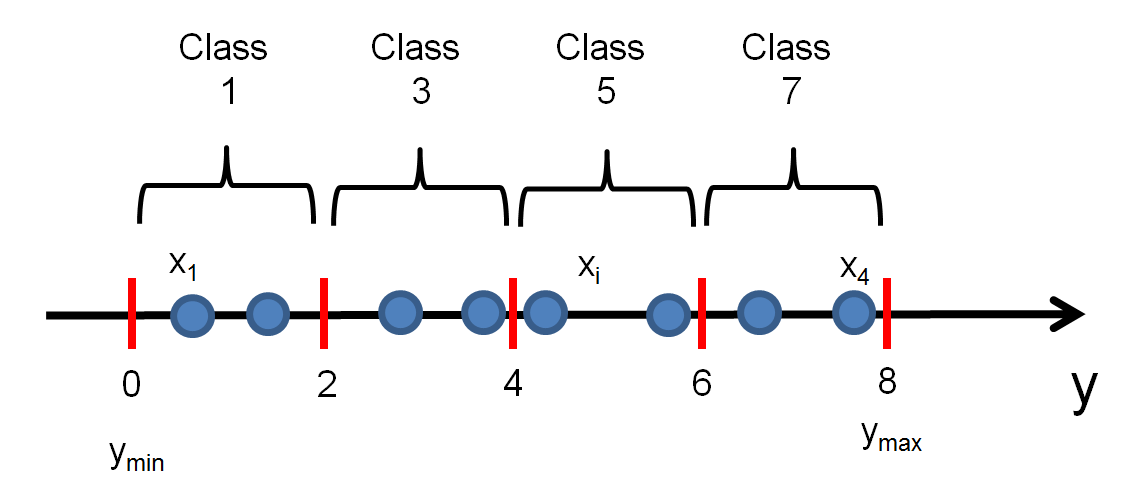
\includegraphics[width=0.6\linewidth]{images/Discretize_binning}
\caption{Example of discretization by binning a continuous label $y$ into $Q=4$ equal-length intervals. Each interval is associated to a unique class label. In this example, the class label for each interval is equal to the mean in each interval.}
\label{fig:Discretize_binning}
\end{figure}

\noindent This approach may leads to border effects between the classes. For instance, two samples $\textbf{x}_i$ and $\textbf{x}_j$ that are close to a frontier and that are on different sides of the border will be considered as different, as illustrated in Fig \ref{fig:Discretize_binning_border_effect}. Moreover, a new sample $\textbf{x}_j$ will have its labels $y_j$ assigned to a class and not a real continuous value. 

\begin{figure}[h!]
	\centering
	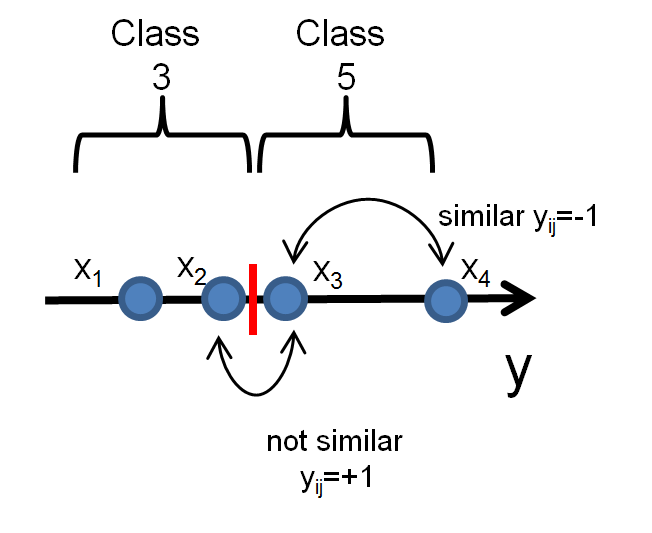
\includegraphics[width=0.42\linewidth]{images/Discretize_binning_border_effect}
	\caption{Border effect problems. In this example, $\textbf{x}_2$ and $\textbf{x}_3$ have closer value labels $y_2$ and $y_3$ than $\textbf{x}_3$ and $\textbf{x}_4$. However, with the discretization $\textbf{x}_2$ and $\textbf{x}_3$ don't belong to the same class and thus are consider as not similar.}
	\label{fig:Discretize_binning_border_effect}
\end{figure}

\noindent The second approach considers the continuous value of $y_i$, computes a $L_1$-norm between the labels $|y_i-y_j|$ and compare this value to a threshold $\epsilon$. Geometrically, a tube of size $\epsilon$ around each value of $y_i$ is built. Two samples $\textbf{x}_i$ and  $\textbf{x}_j$ are considered as similar if the absolute difference between their labels $|y_i-y_j|$ is lower than $\epsilon$ (Fig. \ref{fig:pairwise_label_tube}):
\begin{equation}
y_{ij} = 
\left\{
\begin{split}
\begin{aligned}
-1 & \text{\quad if } |y_i-y_j| \leq \epsilon \\ 
+1 & \text{\quad otherwise }
\end{aligned} 
\end{split}
\right.
\end{equation}

\begin{figure}[h!]
\centering
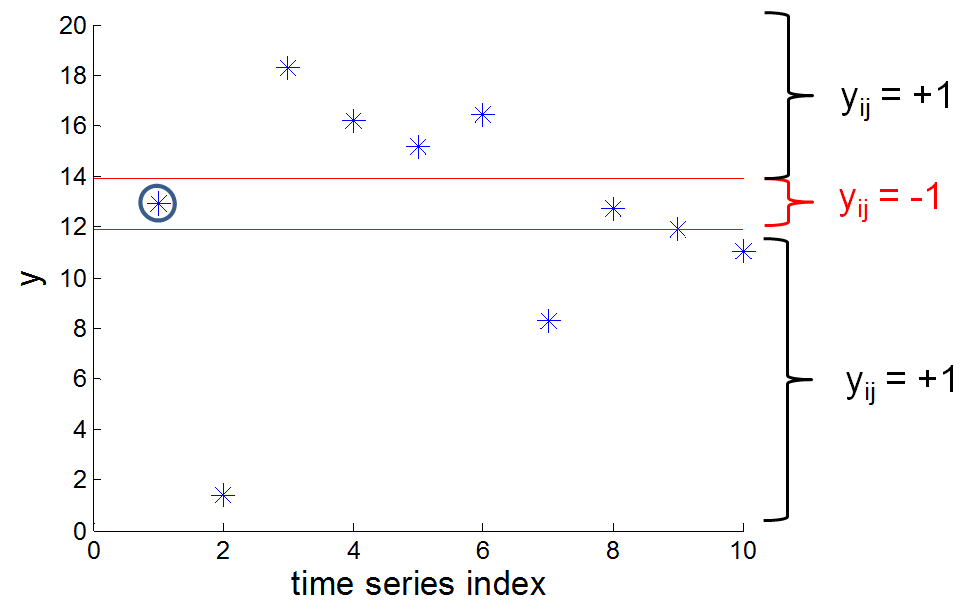
\includegraphics[width=0.65\linewidth]{images/pairwise_label_tube}
\caption{Example of pairwise label definition using an $\epsilon$-tube (red lines) around the time series $\textbf{x}_i$ (circled in blue). For, time series $\textbf{x}_j$ that falls into the tube, the pairwise label is $y_{ij} = -1$ (similar) and outside of the tube, $y_{ij} = +1$ (not similar).}
\label{fig:pairwise_label_tube}
\end{figure}


%---------------------------------------------------------------------------
\subsection{Interpretation in the pairwise space}
%\begin{itemize}
%	\item Proximity to the origin (les individus sont identiques)
%	\item Proximity of 2 pairwise points in the pairwise space 
%	\item Norm in the pairwise space
%	\item Representation of combined metric in the pairwise space
%	\item perte de la classe initiale des individus. L'information qui nous reste est : les 2 individus sont de la même classe ou sont de classes différentes.
%\end{itemize}

The interpretation of the data in the pairwise space is particular since the pairwise space is not a standard Euclidean space. The interpretation in this space requires to be careful.

If $\textbf{x}_{ij}=\textbf{0}$ then $\textbf{x}_{j}$ is identical to $\textbf{x}_{i}$ according to all metrics $d_h$. The norm of the vector $\textbf{x}_{ij}$ can be interpreted as a proximity measure: the lower the norm of $\textbf{x}_{ij}$ is, the closer are the time series $\textbf{x}_{i}$ and $\textbf{x}_{j}$. Nevertheless, if two pairwise vectors $\textbf{x}_{ij}$ and $\textbf{x}_{kl}$ has their norms closed, it doesn't mean that the time series $\textbf{x}_{i}$, $\textbf{x}_{j}$, $\textbf{x}_{k}$ and $\textbf{x}_{l}$ are similar. Fig \ref{fig:ContreExample} shows an example of two pairwise vectors $\textbf{x}_{ij}$ and $\textbf{x}_{kl}$ that are close together in the pairwise space. However, in the temporal space, the time series $\textbf{x}_{1}$ and $\textbf{x}_{3}$ are not similar for example. It means that $\textbf{x}_i$ is as similar to $\textbf{x}_j$ as $\textbf{x}_k$ is to $\textbf{x}_l$.

\begin{figure}[h!]
\centering
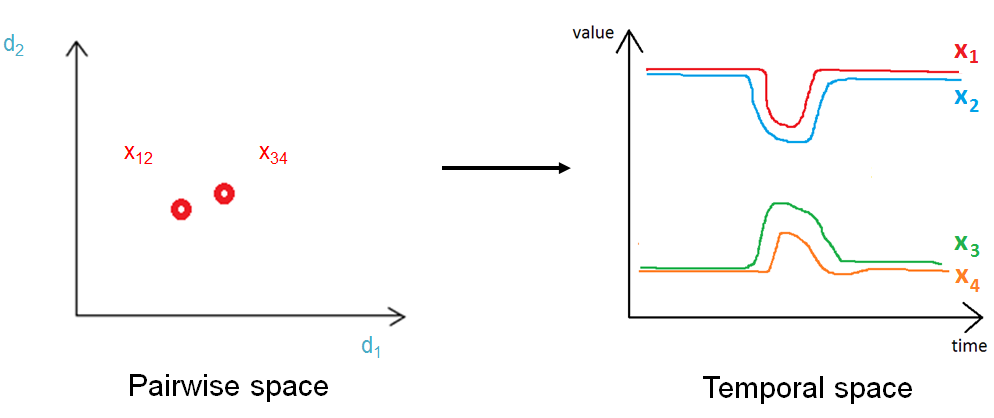
\includegraphics[width=1\linewidth]{images/ContreExample}
\caption{Example of two pairwise vectors $\textbf{x}_{12}$ and $\textbf{x}_{34}$ close in the pairwise space. However, the time series $\textbf{x}_{1}$ and $\textbf{x}_{3}$ are not similar in the temporal space.}
\label{fig:ContreExample}
\end{figure}

A metric $D$ that combines the $p$ unimodal metrics $d_1, \ldots, d_p$ can be seen as a function of the pairwise space. It can be noticed that when the time series $\textbf{x}_i$ are embedded in the pairwise, the information of their original class $y_i$ is lost. Any multi-class problem is transformed in the pairwise space as a binary classification problem.

In the next sections, we transpose the metric learning problem for large margin nearest neighbors in the pairwise space. We propose three formulations: Linear programming, Quadratic programming and {\sc svm}-based approach.

% Fig. \ref{fig:ContourLine} has shown the example of the representation of different combined metrics (linear ($D_{Lin}$), exponential ($D_{Exp}$) and sigmoid ($D_{Sig}$)) in the pairwise space for two modalities: amplitude-based ($d_A$) and behavior-based ($d_B$ and $cort$). 

\section{Linear Programming ({\sc lp}) formalization}
%\begin{itemize}
%	\item Formaliser le problème sous forme d'un problème d'optimisation sous contraintes
%\end{itemize}

Our objective is to define a metric $D$ as a linear combination of the unimodal metric $d_h$ (Eq. \ref{eq:D_linear}). In the pairwise space, the metric $D$ should:
\begin{itemize}
	\item \textbf{pull} to the origin the $k$ nearest neighbors pairs $\textbf{x}_{ij}$ of same labels ($y_{ij}=-1$)
	\item \textbf{push} from the origin all the pairs $\textbf{x}_{il}$ of different classes ($y_{il}=+1$)
\end{itemize}
Fig. \ref{fig:Transposition_Pairwise} illustrates our idea. For each time series $\textbf{x}_i$, we build the set of target pairs $\textbf{x}_{ij}$ ($j \rightsquigarrow i$) and the set of pairs $\textbf{x}_{il}$ of different class ($y_{il}=+1$). Then, we optimise the weight vector $\textbf{w}$ so that the pairs $\textbf{x}_{ij}$ are pulled to the origin and the pairs $\textbf{x}_{il}$ are pushed from the origin.

\begin{figure}[h!]
	\centering
	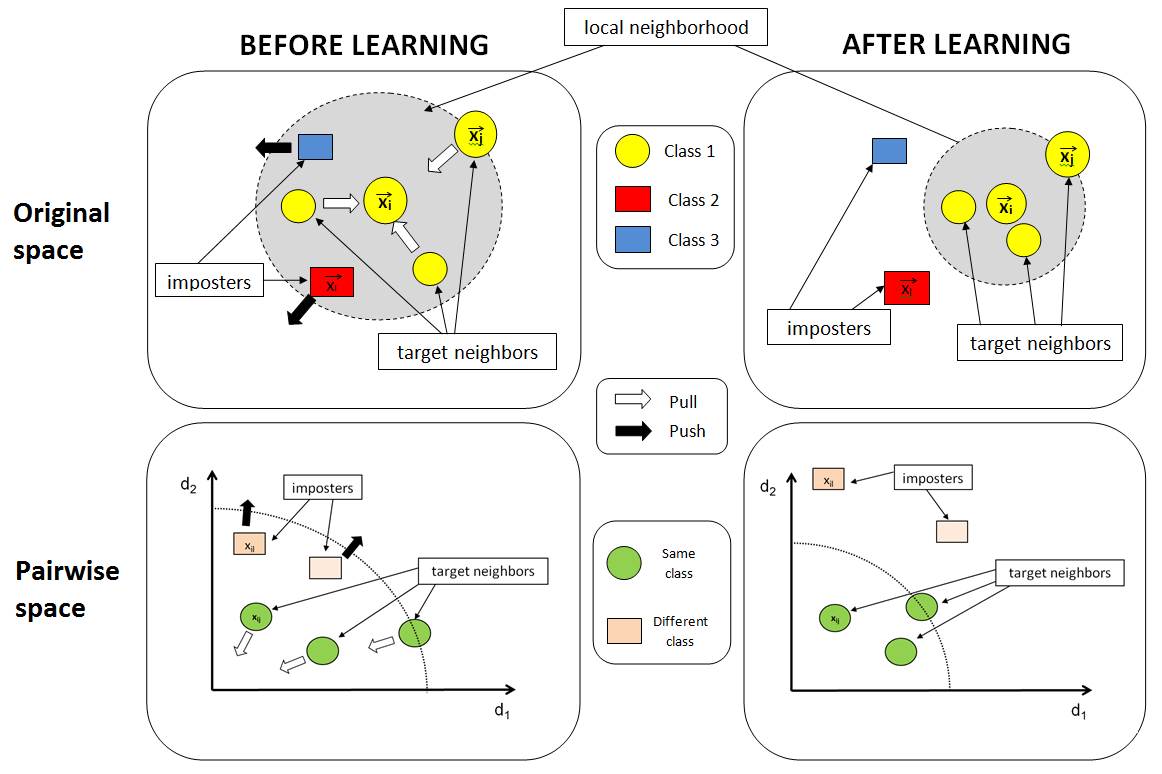
\includegraphics[width=0.9\linewidth]{images/Transposition_Pairwise}
	\caption{Geometric representation of the adaptation of metric learning problem from the original space (top) to the pairwise space (bottom) for a $k=3$ target neighborhood of $\textbf{x}_i$. Before learning (left), imposters $\textbf{x}_l$ invade the targets perimeter $\textbf{x}_j$. In the pairwise space, this is equivalent to have pairwise vectors $\textbf{x}_{il}$ with a norm lower to some pairwise target $\textbf{x}_{ij}$. The aim of metric learning is to push pairwise $\textbf{x}_{il}$ (black arrow) and pull pairwise $\textbf{x}_{ij}$ from the origin (white arrow).}
	\label{fig:Transposition_Pairwise}
\end{figure}

Inspired from the Large Margin Nearest Neighbors ({\sc lmnn}) framework proposed by Weinberger \& Saul in Section \ref{LMNN}, we transpose the metric learning problem into the pairwise space to learn a temporal metric $D$ combining several unimodal metric $d_h$. In our problem, the optimal metric $D$ is learned as the solution of a minimization problem, such that for each time series $\textbf{x}_i$, it pulls its targets $\textbf{x}_j$ and pushes all the samples $\textbf{x}_l$ with a different label ($y_l \neq y_i$). The Time series Metric Learning ({\sc tml}) problem in the pairwise space is formalized as:
\begin{align}
	&\displaystyle 		\argmin_{D,\xi} \left\lbrace \underbrace{
		\vphantom{ \sum\limits_{i,j \rightsquigarrow i,l} \frac{1+y_{il}}{2}.\xi_{ijl} }
		\sum_{i,j\rightsquigarrow i}D(\textbf{x}_{ij})
	}_{pull}
	+
	\underbrace{
		C\sum\limits_{i,j \rightsquigarrow i,l} \frac{1+y_{il}}{2}.\xi_{ijl}
	}
	_{push} \right\rbrace  \label{eq:OriginalOptimizationProblem_Objective} \\
	&\text{s.t.  } \forall j \rightsquigarrow i, y_l\neq y_i, \nonumber \\
	& \qquad D(\textbf{x}_{il})-D(\textbf{x}_{ij}) \geq 1-\xi_{ijl} \label{eq:OriginalOptimizationProblem2}\\
	& \qquad \xi_{ijl} \geq 0 
	\label{eq:OriginalOptimizationProblem} 
\end{align}

\noindent where $\xi_{ijl}$ are the slack variables and $C$, the trade-off between the pull and push costs. The proposed {\sc tml} differs from {\sc lmnn} in which the push term in {\sc tml} considers all samples $\textbf{x}_l$ with a different label from $\textbf{x}_i$, whereas in {\sc lmnn}, only the imposters are taken into consideration (those whose invade the target perimeter). Intuitively, this due to the fact that we do not want that samples $\textbf{x}_l$ with a different class that were not at the beginning imposters, become imposters during the optimization process. By considering all the samples $\textbf{x}_l$, we ensure that at each step of the optimization process, if a sample $\textbf{x}_l$ becomes an imposter, then it will violate the constraints in Eq. \ref{eq:OriginalOptimizationProblem} and thus, its slack variables $\xi_{ijl}$ will be penalized in the objective function (Eq. \ref{eq:OriginalOptimizationProblem_Objective}) :
\begin{itemize}
	\item If $D(\textbf{x}_{il}) < D(\textbf{x}_{ij})$, then the pairs $\textbf{x}_{il}$ is an imposter pair that invades the neighborhood of the target pairs $\textbf{x}_{ij}$. The slack variable  $\xi_{ijl} > 1$ will be penalized in the objective function (Eq. \ref{eq:OriginalOptimizationProblem_Objective}). 
	\item If $D(\textbf{x}_{il}) \geq D(\textbf{x}_{ij})$ but $D(\textbf{x}_{il}) \leq D(\textbf{x}_{ij})+1$, the pair $\textbf{x}_{il}$ is within the safety margin of the target pairs $\textbf{x}_{ij}$. The slack variable $ \xi_{ijl} \in [0;1]$ will have a small penalization effect in the objective function (Eq. \ref{eq:OriginalOptimizationProblem_Objective}).
	\item If $D(\textbf{x}_{il}) > D(\textbf{x}_{ij}) +1$, $\xi_{ijl} = 0$ and the slack variable has no effect in the objective function (Eq. \ref{eq:OriginalOptimizationProblem_Objective}).
\end{itemize}
\noindent By considering a linear combination of the unimodal distance $d_h$ (Chapter \ref{sec:Chapter_metrics}): $D(\textbf{x}_i,\textbf{x}_j) = \sum_h w_h.d_h(\textbf{x}_i,\textbf{x}_j)$, optimizing the metric $D$ is equivalent to optimizing the weight vector $\textbf{w}$. Eqs. \ref{eq:OriginalOptimizationProblem_Objective} and \ref{eq:OriginalOptimizationProblem2} leads to the {\sc tml} primal formulation:
		\begin{align}
		&\displaystyle 		\argmin_{\textbf{w},\xi}
		\left\lbrace \underbrace{
		\vphantom{ \sum\limits_{i,j \rightsquigarrow i,l} \frac{1+y_{il}}{2}.\xi_{ijl} }
			||\textbf{X}_{tar}^T \textbf{w}||	
		}_{pull}					
		+	
		C \underbrace{				
			\sum\limits_{i,j \rightsquigarrow i,l} \frac{1+y_{il}}{2}.\xi_{ijl}
		}_{push} \right\rbrace \label{eq:MMLPrimal} \\
		&\text{s.t.  } \forall j \rightsquigarrow i, y_l\neq y_i, \nonumber \\
		& \qquad \textbf{w}^T(\textbf{x}_{il}-\textbf{x}_{ij}) \geq 1-\xi_{ijl} \label{eq:MMLPrimal_constraint1} \\
		& \qquad \xi_{ijl} \geq 0
		\label{eq:MMLPrimal_constraint2}
		\end{align}
\noindent where $\textbf{X}_{tar}$ is a $p \times (k.N)$ matrix  containing all targets $\textbf{x}_{ij}$ and $||\textbf{X}_{tar}^T \textbf{w}||$ denotes the norm of the vector $\textbf{X}_{tar}^T \textbf{w}$. As in {\sc svm}, a $L_1$ or $L_2$ norm can be chosen. $L_1$ norm will priviledge sparse solution of $\textbf{w}$. \\
{\sc tml} can be seen as a large margin problem in the pairwise space and parallels can be done with {\sc svm}. The "pull" term acts as a regularizer which aims to minimize the norm of $\textbf{w}$. Similarly to {\sc svm}, mininimizing the norm of $\textbf{w}$ is equivalent to maximizing the margin $\frac{1}{||\textbf{w}||}$ between target pairs $\textbf{x}_{ij}$ and pairs of different class $\textbf{x}_{il}$. 
% To ensure the positivity of the learnt metric $D$ (property 1 in Section \ref{sec:property_metric}), one possible solution is to set $w_h \geq 0$ for all $h=1...p$. This constraint can be added into the optimization problem.

\section{Quadratic Programming ({\sc qp}) formalization}
%\begin{itemize}
%	\item Passer de la forme LP (forme primale) et par transformation, arriver à la forme duale
%	\item Montrer les similitudes avec la résolution {\sc svm}
%	\item Montrer que l'on peut kerneliser la méthode
%\end{itemize}
The primal formulation of {\sc tml} (Eqs. \ref{eq:MMLPrimal}, \ref{eq:MMLPrimal_constraint1} and \ref{eq:MMLPrimal_constraint2}) supposed that the metric $D$ is a linear combination of the metrics $d_h$. The primal formulation being similar to the one of {\sc svm}, it can be derived into its dual form to obtain non-linear solutions for $D$.
% Similarly to the SVM dual formulation (Section \ref{sec:dualSVM}), the TML primal formulation in Eq. \ref{eq:MMLPrimal} can be derived into its dual form to obtain non-linear solutions for $D$. 
For that, we consider in the objective function (Eq. \ref{eq:MMLPrimal}), the square of the $L_2$-norm on $\textbf{w}$ as the regularizer term, $\frac{1}{2}||\textbf{X}_{tar}^T \textbf{w}||_2^2$:

\begin{align}
	&\displaystyle 		\argmin_{\textbf{w},\xi}
	\left\lbrace \frac{1}{2}||\textbf{X}_{tar}^T \textbf{w}||_2^2						
	+					
	C\sum\limits_{i,j \rightsquigarrow i,l} \frac{1+y_{il}}{2}.\xi_{ijl}
	\right\rbrace  \label{eq:MMLPrimalL2} \\
	&\text{s.t.  } \forall j \rightsquigarrow i, y_l\neq y_i, \nonumber \\
	& \qquad \textbf{w}^T(\textbf{x}_{il}-\textbf{x}_{ij}) \geq 1-\xi_{ijl} \label{eq:MMLPrimalL2_constraints1} \\
	& \qquad \xi_{ijl} \geq 0 \label{eq:MMLPrimalL2_constraints2}
\end{align}
This formulation can be reduced to the minimization of the following Lagrange function $L(\textbf{w},\xi,\boldsymbol{\alpha},\textbf{r})$, consisting of the sum of the objective function (Eq. \ref{eq:MMLPrimalL2}) and the constraints (Eqs. \ref{eq:MMLPrimalL2_constraints1} and \ref{eq:MMLPrimalL2_constraints2}) multiplied by their respective Lagrange multipliers $\boldsymbol{\alpha}$ and $\textbf{r}$:
\begin{equation}
\begin{aligned}
	L(\textbf{w},\xi,\boldsymbol{\alpha},\textbf{r}) 
	= & 
	\frac{1}{2}||\textbf{X}_{tar}^T \textbf{w}||_2^2
	+ C \sum\limits_{ijl} \frac{1+y_{il}}{2} \xi_{ijl} - \sum\limits_{ijl}r_{ijl} \xi_{ijl} \\
	&  - \sum\limits_{ijl} \alpha_{ijl}\left( \textbf{w}^T(\textbf{x}_{il}-\textbf{x}_{ij}-1+\xi_{ijl} \right))
	\label{eq:OptimizationDual}
\end{aligned}
\end{equation}
\noindent where $\alpha_{ijl} \geq 0$ and $r_{ijl} \geq 0$ are the Lagrange multipliers. At the minimum value of $L(\textbf{w},\xi,\boldsymbol{\alpha},\textbf{r})$, we assume the derivatives with respect to $\textbf{w}$ and $\xi_{ijl}$ are set to zero:
\begin{align*}
\frac{\partial L}{\partial \textbf{w}} 
& = 
\textbf{X}_{tar}^T \textbf{X}_{tar} \textbf{w} 
- \sum\limits_{ijl} \alpha_{ijl}(\textbf{x}_{il}-\textbf{x}_{ij}) 
= 0 \\
\frac{\partial L}{\partial \xi_{ijl}} & = C - \alpha_{ijl} - r_{ijl} = 0
\end{align*}
\noindent that leads to:
\begin{align}
& \textbf{w} = (\textbf{X}_{tar} \textbf{X}_{tar}^T)^{-1}  
\sum\limits_{ijl} \alpha_{ijl}(\textbf{x}_{il}-\textbf{x}_{ij}) \label{Eq:eqn_w} 
\\ 
& r_{ijl} = C - \alpha_{ijl} \label{Eq:eqn_w2}
\end{align}

\noindent Substituting Eq. \ref{Eq:eqn_w} and \ref{Eq:eqn_w2} back into $L(\textbf{w},\xi,\boldsymbol{\alpha},\textbf{r})$ in Eq. \ref{eq:OptimizationDual}, we get the {\sc tml} dual formulation\footnote{complete details of the calculations in Appendix \ref{chap:app:qp_resolution}}:
\begin{align}
&\displaystyle \argmax_{\boldsymbol{\alpha}} \left\lbrace 
\sum\limits_{ijl} \alpha_{ijl} 
- \frac{1}{2} \sum\limits_{ijl} \sum\limits_{i'j'l'}
\alpha_{ijl} \alpha_{i'j'l'}
(\textbf{x}_{il}-\textbf{x}_{ij})^T
(\textbf{X}_{tar} \textbf{X}_{tar}^T)^{-1}
(\textbf{x}_{i'l'}-\textbf{x}_{i'j'}) \right\rbrace \label{eq:OptimDual} \\
&\text{s.t. $\forall$ $i$, $j \rightsquigarrow i$ and $l$ s.t. $y_{il}=+1$:} \nonumber \\
& 0 \leq \alpha_{ijl} \leq C
\label{eq:OptimDualconstraint}
\end{align}

\noindent For any new pair of samples $\textbf{x}_{i'}$ and $\textbf{x}_{j'}$, the resulting metric $D$ writes: 
\begin{align}
D(\textbf{x}_{i'j'}) = & \textbf{w}^T \textbf{x}_{i'j'} \label{eq:D1} \\
D(\textbf{x}_{i'j'}) = & \sum\limits_{ijl} \alpha_{ijl} 
(\textbf{x}_{il}-\textbf{x}_{ij})^T
(\textbf{X}_{tar}\textbf{X}_{tar}^T)^{-1}
\textbf{x}_{i'j'}
\label{eq:D1_2}
\end{align}
% At the optimality, only the triplet $(\textbf{x}_{il}-\textbf{x}_{ij})$ which $\textbf{x}_{il}$ that has the $L_2$ norm greater than 1 and that lies closest to the unit circle of targets $\textbf{x}_{ij}$ or those triplets that have a $L_2$ norm lower that one, have $\alpha_{ijl} > 0$. These points are the support vectors. 
with $\textbf{w}$ defined in Eq. \ref{Eq:eqn_w}. At the optimality, only the triplets $(\textbf{x}_{il}-\textbf{x}_{ij})$ with $\alpha_{ijl} > 0$ are considered as the support vectors. The direction $\textbf{w}$ of the metric $D$ is lead by these triplets. All other triplets have $\alpha_{ijl} = 0$ (non-support vector), and the metric $D$ is independent from this triplets. If we remove some of the non-support vectors, the metric $D$ remains unaffected. From the viewpoint of optimization theory, we can also see this from the Karush-Kuhn-Tucker (KKT) conditions: the complete set of conditions which must be satisfied at the optimum of a constrained optimization problem. At the optimum, the Karush-Kuhn-Tucker (KKT) conditions apply, in particular:
\begin{equation*}
\alpha_{ijl} (\textbf{w}^T (\textbf{x}_{il}-\textbf{x}_{ij}) - 1 + \xi_{ijl}) = 0
\end{equation*}

\noindent from which we deduce that either $\textbf{w}^T(\textbf{x}_{il}-\textbf{x}_{ij}) > 1 $ and $\alpha_{ijl} = 0$ (the triplet $(\textbf{x}_{il}-\textbf{x}_{ij})$ is a non-support vector), or $\textbf{w}^T(\textbf{x}_{il}-\textbf{x}_{ij}) = 1- \xi_{ijl}$ and $\alpha_{ijl} > 0$ (the triplet is a support vector). Therefore, the learned metric $D$ is a combination of scalar products between new pairs $\textbf{x}_{i'j'}$ and a few number of triplets $\textbf{x}_{ijl}$ of the training set. \\


\noindent \textbf{Extension to non-linear function of $D$} \\
\noindent The above formula can extended to non-linear function for the metric $D$. The dual formulation in Eq.~\ref{eq:OptimDual} only relies on the inner product $(\textbf{x}_{i'l'}-\textbf{x}_{i'j'})^T (\textbf{X}_{tar} \textbf{X}_{tar}^T)^{-1} (\textbf{x}_{il}-\textbf{x}_{ij})$. We can hence apply the kernel trick on Eqs. \ref{eq:D1} and \ref{eq:D1_2} to find non-linear solutions for $D$:
\begin{align}
D(\textbf{x}_{i'j'}) & = \textbf{w}^T \phi(\textbf{x}_{i'j'}) \nonumber\\
D(\textbf{x}_{i'j'}) &= \sum\limits_{ijl} \alpha_{ijl} 
\phi(
\textbf{x}_{il}-\textbf{x}_{ij}
)
\phi(	
\textbf{x}_{i'j'}
) \nonumber \\
D(\textbf{x}_{i'j'}) &= \sum\limits_{ijl} \alpha_{ijl} 
K(\textbf{x}_{il}-\textbf{x}_{ij} ; \textbf{x}_{i'j'}) \nonumber				
\end{align}
These equations suppose that the null vector $\textbf{0}$ in the original space is transformed through the transformation $\phi$ into the null vector: $\phi(\textbf{0})=\textbf{0}$ in the feature space. We recall that $D(\textbf{x}_{ii} = \textbf{0})$ is expected to be equal to zero (distinguishability property in Section \ref{sec:property_metric}). However, if the vectors $\textbf{x}_{ij}$ are projected in a feature space by a transformation $\phi$, it doesn't guarantee that $\phi(\textbf{0})=\textbf{0}$. Fig. \ref{fig:Kernel_nonHomogene} illustrates the idea for a polynomial kernel in which $\phi(\textbf{0}) = [0, 0, 0, 1]^T$. Thus, the metric measure needs to be computed in the feature space relatively to the projection of $\phi(\textbf{0})$. This is done by adding a term $\textbf{w}^T \phi(\textbf{0})$ to Eqs. \ref{eq:D1} and \ref{eq:D1_2}:

\begin{align}
D(\textbf{x}_{i'j'}) & = \textbf{w}^T \phi(\textbf{x}_{i'j'}) - \textbf{w}^T \phi(\textbf{0})\\
D(\textbf{x}_{i'j'}) &= \sum\limits_{ijl} \alpha_{ijl} 
\phi(
\textbf{x}_{il}-\textbf{x}_{ij}
)
\phi(	
\textbf{x}_{i'j'}-\textbf{x}_{ij}
) 
-
\sum\limits_{ijl} \alpha_{ijl} 
\phi(
\textbf{x}_{il}-\textbf{x}_{ij}
)
\phi(	
\textbf{0}-\textbf{x}_{ij}
) 				
\\
D(\textbf{x}_{i'j'}) &= \sum\limits_{ijl} \alpha_{ijl} 
K
\left( 
\textbf{x}_{il}-\textbf{x}_{ij}
;	
\textbf{x}_{i'j'}-\textbf{x}_{ij}
\right) 		
-
\sum\limits_{ijl} \alpha_{ijl} 
K
\left( 
\textbf{x}_{il}-\textbf{x}_{ij}
;	
\textbf{0}-\textbf{x}_{ij}
\right) 		
\label{Eq:nonlinearD}		
\end{align}
%For any new pair of samples $\textbf{x}_{i'}$ and $\textbf{x}_{j'}$, the resulting metric $D$ writes: 
%\begin{align}
%D(\textbf{x}_{i'j'}) = & \textbf{w}^T \textbf{x}_{i'j'} - \textbf{w}^T \textbf{0} 
%\nonumber \\
%D(\textbf{x}_{i'j'}) = & \sum\limits_{ijl} \alpha_{ijl} 
%(\textbf{x}_{il}-\textbf{x}_{ij})^T
%(\textbf{X}_{tar}\textbf{X}_{tar}^T)^{-1}
%\textbf{x}_{i'j'} 
%-
%\sum\limits_{ijl} \alpha_{ijl} 
%(\textbf{x}_{il}-\textbf{x}_{ij})^T
%(\textbf{X}_{tar}\textbf{X}_{tar}^T)^{-1}
%\textbf{0}
%\nonumber \\
%& -\sum\limits_{ijl} \alpha_{ijl} 
%(\textbf{x}_{il}-\textbf{x}_{ij})^T
%(\textbf{X}_{tar}\textbf{X}_{tar}^T)^{-1}\textbf{x}_{ij} + \sum\limits_{ijl} \alpha_{ijl} 
%(\textbf{x}_{il}-\textbf{x}_{ij})^T
%(\textbf{X}_{tar}\textbf{X}_{tar}^T)^{-1}\textbf{x}_{ij}
%\nonumber \\
%D(\textbf{x}_{i'j'}) = & \sum\limits_{ijl} \alpha_{ijl} 
%(\textbf{x}_{il}-\textbf{x}_{ij})^T
%(\textbf{X}_{tar}\textbf{X}_{tar}^T)^{-1}
%(\textbf{x}_{i'j'}-\textbf{x}_{ij}) 
%\nonumber \\
%& - \sum\limits_{ijl} \alpha_{ijl} 
%(\textbf{x}_{il}-\textbf{x}_{ij})^T
%(\textbf{X}_{tar}\textbf{X}_{tar}^T)^{-1}
%(\textbf{0}-\textbf{x}_{ij}) \label{eq:D2}
%\end{align}
\noindent where $\textbf{0}$ denotes the null vector. The resulting metric $D$ is made of two terms. The first one, $\textbf{w}^T \phi(\textbf{x}_{i'j'})$, is the metric measure for a new pair $\textbf{x}_{i'j'}$. The second term, $\textbf{w}^T \phi(\textbf{0})$, adapts the metric measure relatively to the origin point. 

\begin{figure}[h!]
\centering
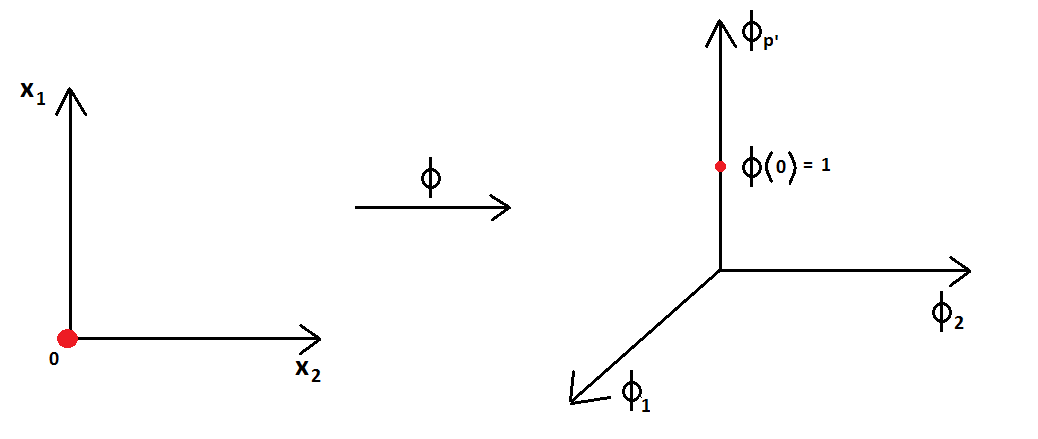
\includegraphics[width=0.9\linewidth]{images/Kernel_nonHomogene}
\caption{Illustration of samples in $\mathbb{R}^2$. The transformation $\phi$ for a polynomial kernel $K(\textbf{x}_i,\textbf{x}_j)=(\textbf{x}_i^T \textbf{x}_j + c)^d$ with $c=1$ and $d=2$ can be written explicitly: $\phi(\textbf{x}_i)= [x_{i1}^2, x_{i2}^2, \sqrt{2} x_{i1} x_{i2}, 1]^T$. The origin point $\textbf{x}_i=[0,0]^T$ is projected in the Hilbert space as $\phi(\textbf{x}_i=\textbf{0}) = [0, 0, 0, 1]^T$.}
\label{fig:Kernel_nonHomogene}
\end{figure}

However, to define proper metrics that respects the properties of metrics (Section \ref{sec:property_metric}), specific kernels must be used. Our work don't propose any solutions to this problem but open the field for new research on this topic. 



\section{Support Vector Machine ({\sc svm}) approximation}
\subsection{Motivations}
%\begin{itemize}
%	\item Faire remarquer que le problème LP ressemble à un problème SVM
%	\item Faire la démonstration de l'équivalence (ou mettre la démonstration en annexe).
%	\item Expliquer les différences entre la résolution LP/QP et la résolution SVM. (ajout de sur-contraintes dans le problème SVM)
%	\item Expliquer pourquoi on va préférer le cadre SVM. Expliquer mathématiquement et avec des interprétations géométriques. 
%	\item Cadre connu
%	\item Utilisation de librairie standard de Machine Learning
%	\item Extension directe à l'apprentissage de métrique non linéaire grâce au kernel trick
%\end{itemize}

Many parallels have been studied between Large Margin Nearest Neighbors ({\sc lmnn}) and {\sc svm} (Section \ref{sec:LMNN_SVM}). Similarly, the proposed {\sc tml} approach can be linked to {\sc svm}: both are convex optimization problem based on a regularized and a loss term. {\sc svm} is a well known framework: its has been well implemented in many libraries (e.g., {\sc liblinear} \cite{Fan2008} and {\sc libsvm} \cite{Hsu2008}), well studied for its generalization properties and extension to non-linear solutions. \\
\indent Motivated by these advantages, we propose to solve the {\sc tml} problem by solving a similar {\sc svm} problem. Then, we can naturally extend {\sc tml} approach to find non-linear solutions for the metric $D$ thanks to the 'kernel trick'. 
In the following, we show the similarities and the differences between {\sc lp}/{\sc qp} and {\sc svm} formulation.

For a time series $\textbf{x}_i$, we define the set of pairs $\textbf{X}_{pi}=\{(\textbf{x}_{ij},y_{ij}) \text{ s.t. } j\rightsquigarrow i \text{ or } y_{ij}=+1\}$. It corresponds for a time series $\textbf{x}_i$ to the set of pairs with target samples $\textbf{x}_j$ ($k$ nearest samples of same labels $j\rightsquigarrow i$) or samples $\textbf{x}_l$ that has a different label from $\textbf{x}_i$ ($y_l \neq y_i$) . Identity pairs $\textbf{x}_{ii}$ are not considered. We refer to $\textbf{X}_{p}=\bigcup\limits_{i} \textbf{X}_{pi}$ and consider the following standard soft-margin weighted {\sc svm} problem on $\textbf{X}_p$ \footnote{the {\sc svm} formulation below divides the loss part into two terms similarly to asymetric {\sc svm}}: 
\begin{equation}
\begin{aligned}
&\displaystyle \argmin_{\textbf{w},b,\xi} 
\left\lbrace \frac{1}{2}||\textbf{w}||_2^2
+ C \sum\limits_{i,j,y_{ij=-1}}p_i^-\xi_{ij}
+ C \sum\limits_{i,j, y_{ij=+1}}p_i^+\xi_{ij} \right\rbrace \\
& \text{s.t.  }  y_{ij}(\textbf{w}^T\textbf{x}_{ij}+b) \geq 1-\xi_{ij}
\end{aligned}
\label{eq:SVMSofMarginProblem}
\end{equation}
\noindent where $p_i^-$ and $p_i^+$ are the weight factors for target pairs and pairs of different class.

\noindent  We show in the following that solving the {\sc svm} problem in Eq.~\ref{eq:SVMSofMarginProblem} for $\textbf{w}$ and $b$ solves a similar {\sc tml} problem in Eq.~\ref{eq:MMLPrimalL2} for $D(\textbf{x}_i,\textbf{x}_j)=\frac{1}{2}(\textbf{w}^T\textbf{x}_{ij}+b)$. If we set $p_i^+$ being the half of the number of targets of $\textbf{x}_i$ and $p_i^-$, the half of the number of time series $L$ of a different class than $\textbf{x}_i$:
\begin{align}
p_i^+ &= \frac{k}{2} = \sum_{j \rightsquigarrow i} \frac{1}{2} \label{eq:pi_plus}\\
p_i^- &= \frac{L}{2} = \frac{1}{2}\sum_l \frac{1+y_{il}}{2} \label{eq:pi_moins}
\end{align}
% \noindent Note that in the case of $Q$ balanced classes of size $N$,  $p_i^- = N (Q-1)$. 

\subsection{Similarities and differences in the constraints}
% \noindent \textbf{Equivalence in the constraints} \\
\noindent First, we recall the {\sc svm} constraints in Eq.~\ref{eq:SVMSofMarginProblem}:
\begin{equation*}
y_{ij}(\textbf{w}^T\textbf{x}_{ij}+b) \geq 1-\xi_{ij} 
\end{equation*}
\noindent These constraints can be split into two sets of constraints:
%\begin{equation*}
%\begin{aligned}
%y_{ij}(\textbf{w}^T\textbf{x}_{ij}+b) & \geq 1-\xi_{ij} \text{ \quad (same class)} \\
%y_{il}(\textbf{w}^T\textbf{x}_{il}+b) & \geq 1-\xi_{il} \text{ \quad  (different classes)}
%\end{aligned}
%\end{equation*}
%\noindent which is equivalent to:
\begin{equation*}
\begin{aligned}
-(\textbf{w}^T\textbf{x}_{ij}+b) & \geq 1-\xi_{ij} \text{ \quad (same class: $y_{ij}=-1$)} \\
(\textbf{w}^T\textbf{x}_{il}+b) & \geq 1-\xi_{il} \text{ \quad  (different classes: $y_{ij}=+1$)}
\end{aligned}
\end{equation*}
\noindent By defining $D(\textbf{x}_{ij})=\frac{1}{2}(\textbf{w}^T\textbf{x}_{ij}+b)$, this leads to:
\begin{equation*}
\begin{aligned}
-D(\textbf{x}_{ij}) & \geq \frac{1}{2}-\frac{\xi_{ij}}{2} \\
D(\textbf{x}_{il}) & \geq \frac{1}{2}-\frac{\xi_{il}}{2}
\end{aligned}
\end{equation*}  
\noindent By summing each constraint two by two, this set of constraints implies the following set of constraints: \\
\resizebox{1\linewidth}{!}{
	\begin{minipage}{\linewidth}
		\begin{eqnarray}
		\begin{cases}
		\bullet \forall i,j,k,l \text{ such that } y_{ij}=-1, \text{ and } y_{kl}=+1, i \neq j \text{ and } i \neq k: \\
		D(\textbf{x}_k,\textbf{x}_l)-D(\textbf{x}_i,\textbf{x}_j) \geq 1-\frac{\xi_{kl}+\xi_{ij}}{2}  \\
		\bullet \forall i,j,l \text{ such that } y_{ij}=-1, \text{ and } y_{il}=+1, i \neq j: \\
		D(\textbf{x}_i,\textbf{x}_l)-D(\textbf{x}_i,\textbf{x}_j) \geq 1-\frac{\xi_{il}+\xi_{ij}}{2}
		\end{cases}
		\label{eq:Rewriten_Constraints}
		\end{eqnarray}
	\end{minipage}
} \\

\noindent By defining $\xi_{ijl}=\frac{\xi_{ij}+\xi_{il}}{2}$, the second constraint in Eq.~\ref{eq:Rewriten_Constraints} from the {\sc svm} formulation is the same as the constraints in the {\sc tml} formulation in Eq.~\ref{eq:MMLPrimalL2_constraints1}. 

\indent However, an additional set of constraints is present in the {\sc svm} formulation (first set of constraints in Eq.~\ref{eq:Rewriten_Constraints}) and not in the proposed {\sc tml}. Geometrically, this can be interpreted as superposing the neighborhoods of all samples $\textbf{x}_i$, making the union of all of their target sets $\textbf{X}_{pi}$, and then pushing away all imposters $\textbf{x}_{il}$ from this resulting target set. This is therefore creating "artificial imposters" $\textbf{x}_{kl}$ that don't violate the local target space of sample $\textbf{x}_k$, but are still considered as imposters because they invade the target of sample $\textbf{x}_i$ (because of the neighborhoods superposition) (Figure \ref{fig:Neighborhood_scaling_problem}). This is more constraining in the {\sc svm} resolution for the resulting metric $D$ especially if the neighborhoods have different spread. 
% To overcome this issue, we propose to scale all target spheres to 1 in the preprocessing set, such that the risk of over-constraining the problem is very much mitigated.

\begin{figure}[h!]
	\centering
	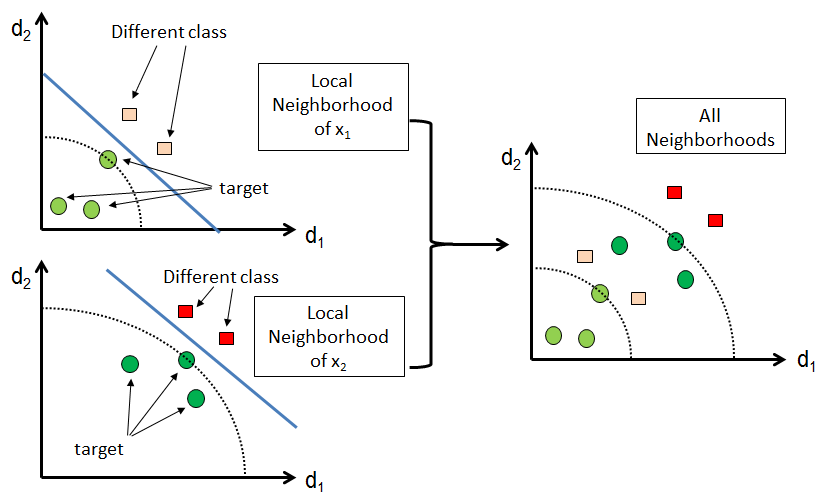
\includegraphics[width=0.9\linewidth]{images/Neighborhood_scaling_problem}
	\caption{Geometric representation of the neighborhood of $k=3$ for two time series $\textbf{x}_1$ and $\textbf{x}_2$ (left). For each neighborhood, time series of different class are represented by a square and the margin by a blue line. Taking each neighborhood separately, the problem is linearly separable ({\sc lp}/{\sc qp} formulation). By combining the two neighborhoods ({\sc svm} formulation), the problem is no more linearly separable and in this example, the time series of different class of $\textbf{x}_1$ (orange square) are "artificial imposters" of $\textbf{x}_2$. }
	\label{fig:Neighborhood_scaling_problem}
\end{figure}


\subsection{Similarities and differences in the objective function}
\label{sec:relationship}

% \noindent \textbf{Equivalence in the objective function} \\
\noindent Mathematically, from Eq. \ref{eq:pi_plus}, we write:
%\begin{equation}
\begin{align}
\sum\limits_{i,l,y_{il=+1}}p_i^+\xi_{il} 
& = 
\sum_{il}p_i^+   \frac{1+y_{il}}{2}  \xi_{il} \nonumber\\
& = 
\sum_{il} \left( \sum_{j \rightsquigarrow i} \frac{1}{2}\right)  \frac{1+y_{il}}{2}  \xi_{il} \nonumber\\
& =
\frac{1}{2}\sum_{i,j \rightsquigarrow i, l} \frac{1+y_{il}}{2}\xi_{il} \label{eq:pi_plus2}
\end{align}
%\end{equation}

\noindent And from Eq. \ref{eq:pi_moins}, we write:
\begin{align}
\sum\limits_{i,j, y_{ij=-1}}p_i^-\xi_{ij} 
& = 
\sum_{i,j \rightsquigarrow i}p_i^-\xi_{ij} \nonumber \\
& =
\sum_{i,j \rightsquigarrow i} \left( \frac{1}{2}\sum_l \frac{1+y_{il}}{2} \right) \xi_{ij} \nonumber \\
& =
\frac{1}{2}\sum_{i,j \rightsquigarrow i, l} \frac{1+y_{il}}{2}\xi_{ij} \label{eq:pi_moins2}
\end{align}

\noindent By replacing Eqs. \ref{eq:pi_plus2} and \ref{eq:pi_moins2} back into Eq. \ref{eq:SVMSofMarginProblem}, the objective function becomes:
%\begin{equation}
\begin{align}
&\displaystyle \min_{\textbf{w},\xi} 
\frac{1}{2}\textbf{w}^T \textbf{w}
 + C\sum_{i,j \rightsquigarrow i ,l}\frac{1+y_{il}}{2}\frac{\xi_{ij}+\xi_{il}}{2} \nonumber \\
&\displaystyle \min_{\textbf{w},\xi} 
\underbrace{ 
	\vphantom{ \sum\limits_{i,j \rightsquigarrow i,l} }
	\frac{1}{2}\textbf{w}^T \textbf{w}
}_{Regularization}
 + C \underbrace{
	\sum_{i,j \rightsquigarrow i ,l}
	\frac{1+y_{il}}{2} \xi_{ijl} 
}_{Loss}
\label{eq:svm2}
\end{align}	
%\end{equation} 
%\noindent The loss-function part of the {\sc svm} problem is similar to the one in Eq.~\ref{eq:MMLPrimalL2}. We can therefore use such {\sc svm}s with kernels to find non-linear forms for the metric $D$:
%
%\begin{align}
%D(\textbf{x}_{i'},\textbf{x}_{j'}) &= \frac{1}{2} 
%\left( \sum\limits_{ij} \alpha_{ij} 	
%y_{ij} 
%K
%\left( 
%\textbf{x}_{ij}
%,	
%\textbf{x}_{i'j'}
%\right) 
%+ b \right) 
%\label{Eq:nonlinearDSVM}		
%\end{align}

%In this section, we investigate the similarities and the differences between the {\sc lp}/{\sc qp} and {\sc svm} formulations. \\
\indent Even if the loss part (push cost) is the same for both objective functions, the regularization part (pull cost) is different. In the {\sc svm} formulation (Eq. \ref{eq:svm2}), the regularization part tends to minimize the norm of $\textbf{w}$ whereas in {\sc tml} (Eq.~\ref{eq:MMLPrimalL2}), it tends to minimize the norm of $\textbf{w}$ after a linear transformation through $\textbf{X}_{tar}$. This transformation can be interpreted as a Mahalanobis norm in the pairwise space with $\textbf{M}=\textbf{X}_{tar}\textbf{X}_{tar}^T$. Nevertheless, both have the same objective: improve the conditioning of the problem by enforcing solutions with small norms. In practice, even with these differences, the {\sc svm} provides suitable solutions for our time series metric learning problem. \\
%($\textbf{X}_{tar}.\textbf{X}_{tar}^T$ can be seen as a specific choice of Tikhonov matrix). 


\newpage
\subsection{Geometric interpretation}
\todo[inline]{Michèle pense que l'état, cette section est dure à comprendre. D'après Michèle, il faut 1) soit prendre + de place pour expliquer la signification géométrique 2) ou soit ne pas mettre cette partie car étant compliquée, cela pourrait nuire au lecteur. Qu'en penses tu Ahlame?}
In this section, we give a geometric understanding of the differences between {\sc lp}/{\sc qp} resolution (left) and {\sc svm}-based resolution (right). Fig. \ref{fig:Linear} shows the Linear Programming ({\sc lp}) and {\sc svm} resolutions of a $k$-NN problem with $k=2$ neighborhoods. \\

For {\sc lp}, the problem is solved for each neighborhood (blue and red) independently as shown in Fig. \ref{fig:LP_separate}. We recall that {\sc lp}/{\sc qp} resolutions, support vectors are triplets of time series made of a target pair $\textbf{x}_{ij}$ and a pair of different classes $\textbf{x}_{il}$ (black arrows). Support vectors represent triplet which resulting distance $D(\textbf{x}_{ij}, \textbf{x}_{il})$ are the lowest. The optimization problem tends to maximize the margin between these triplets. The global solution (Fig. \ref{fig:Linear} (left)) is a compromise of all of the considered margins. In this case, the global margin is equal to one of the local margin. Note that the global {\sc lp} solution is not always the same as the best local solution. For {\sc svm}-based resolution (Fig. \ref{fig:Linear} (right)), the problem involves all pairs and the margin is optimized so that pairs $\textbf{x}_{ij}$ and $\textbf{x}_{il}$ are globally separated.



\begin{figure}[h!]
	\centering
	\begin{minipage}[b]{1\linewidth}
		\centerline{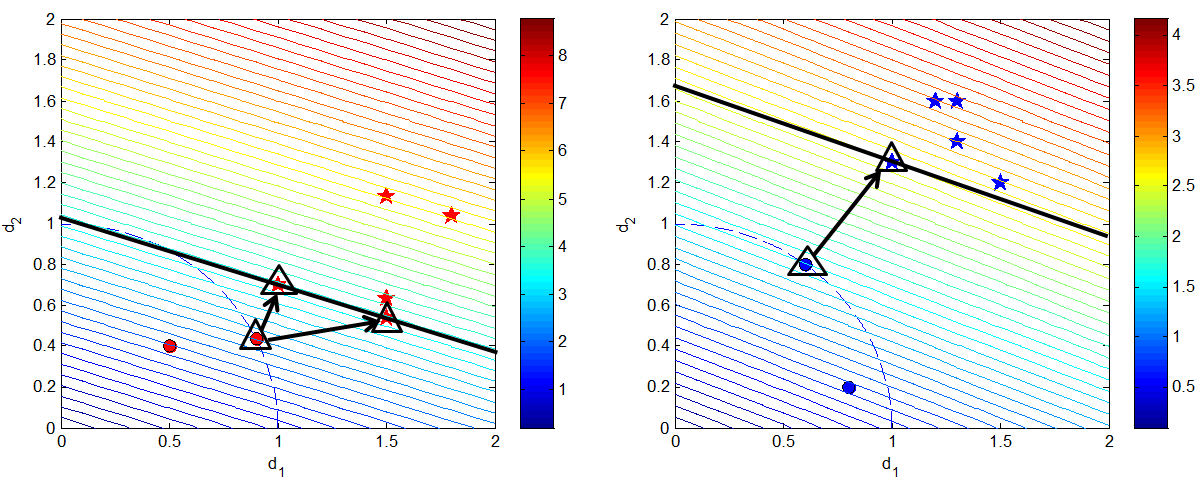
\includegraphics[width=1\linewidth]{images/InterpretationLP}}
	\end{minipage}
	\caption{Solutions found by solving the {\sc lp} problem for $k=2$ neighborhood. Positive pairs (different classes) are indicated in stars and negative pairs (target pairs) are indicated in circle. Red and blue lines shows the margin when solving the problem for each neighborhood (red and blue points) separately. Support vector are indicated in black triangles: in the red neighborhood (left), 2 support vectors are retained and in the blue neighborhood (right), only one support vector is necessary.}
	\label{fig:LP_separate}
\end{figure}

\begin{figure}[h!]
	\centering
	\begin{minipage}[b]{1\linewidth}
		\centerline{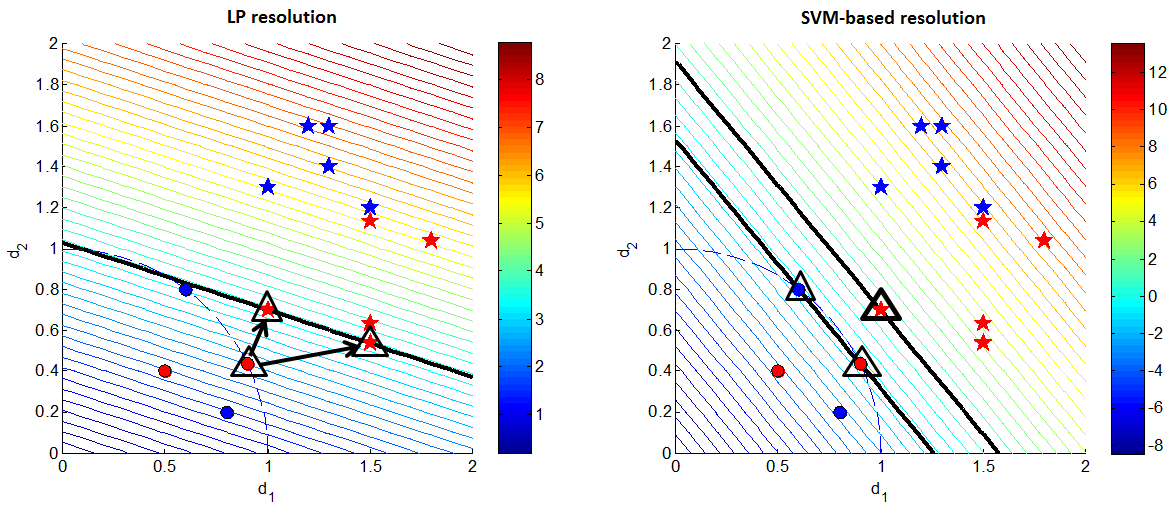
\includegraphics[width=1\linewidth]{images/InterpretationLP_SVM}}
	\end{minipage}
	\caption{Solutions found by solving the {\sc lp} problem (left) and the {\sc svm} problem (right). The global margin is indicated in black and the metric is represented in color levels. Support vectors made of triplets are indicated in black triangles. For the {\sc svm}, the black lines indicates the {\sc svm} canonical hyperplan where the support vector lies (black triangles).}
	\label{fig:Linear}
\end{figure}

\newpage
\section{Conclusion of the chapter}
To learn a combined metric $D$ from several unimodal metrics $d_h$ that optimizes the $k$-NN performances, we first proposed a new space representation, the pairwise space where each pair of time series is projected as a vector described the unimodal metrics. Then, we propose three formalizations of our metric learning problem: Linear Programming, Quadratic Programming, {\sc svm}-based approximation.

In the following, we consider the {\sc svm}-based approximation because {\sc svm} framework is well known and well implementated. In the next chapter, we give the details of the steps of our proposed algorithm: Multi-modal and Multi-scale Time series Metric Learning ({\sc m}$^2${\sc tml}).